\documentclass[8pt]{beamer}
\usetheme{default} % Very simple theme
\usecolortheme{dove} % Minimalist grayscale colors
\setbeamertemplate{navigation symbols}{} % Remove navigation bar

% Define brand-like colors
\definecolor{myblue}{RGB}{0, 102, 204}    % Blue for standard blocks
\definecolor{mygreen}{RGB}{0, 153, 0}     % Green for example blocks
\definecolor{myred}{RGB}{204, 0, 0}       % Red for alert blocks
\definecolor{myorange}{RGB}{255, 128, 0} % For \emph

% Accent color for titles, bullets, etc.
\setbeamercolor{structure}{fg=myblue}

% Block colors
\setbeamercolor{block title}{bg=myblue, fg=white}
\setbeamercolor{block body}{bg=blue!5, fg=black}

\setbeamercolor{exampleblock title}{bg=mygreen, fg=white}
\setbeamercolor{exampleblock body}{bg=green!5, fg=black}

\setbeamercolor{alertblock title}{bg=myred, fg=white}
\setbeamercolor{alertblock body}{bg=red!5, fg=black}
\setbeamercolor{alerted text}{fg=myred}

% Optional: color for \example text
\setbeamercolor{example text}{fg=mygreen}

% Custom emph (orange text instead of italic)
\let\oldemph\emph
\renewcommand{\emph}[1]{\textcolor{myorange}{#1}}


\usepackage{graphicx} % Package for images
\usepackage{amsmath} % Package for images
\graphicspath{{figs/}} % Path to your figures directory
\usepackage{array}  % For better column spacing
\usepackage{caption} % Required for \captionof

% Title Information
\title{STOCHASTIC METHODS IN WATER RESOURCES}
\vspace{25pt}
\subtitle{Unit 4: Time series analysis \\ Lecture 12: Univariate, linear stochastic models}
\author{Luis Alejandro Morales, Ph.D.}
\institute{Universidad Nacional de Colombia \\ Department of Civil and Agriculture Engineering} %// }
%\date{\today}

\begin{document}

% Title Slide
\begin{frame}
    \titlepage
\end{frame}

%-------
% From Kotte (Stochastic WR tech)
\section{Introduction}
\begin{frame}{Introduction}
    \begin{itemize}
        \item Here we will dealt with \alert{univariate linear models} used to represent \emph{stochastic process}. The main purpose of this models is to generate likely \emph{future sequences of data} for \emph{design} and \emph{planning}.
        \item \emph{Generated data sequences} are particularly useful in determining the \emph{reliabilities} of maintaining \emph{specific conditions} from complex systems.
        \item In general, the models are formulated so that the current value of a variable is the \emph{weighted sum} of \emph{past values} and \emph{random numbers} which represent unknown effects. 
    \item Models such \emph{autoregressive (AR)}, \emph{moving average (MA)} and \emph{Box-Jenkins autoregressive moving average (ARMA)} and \emph{autoregressive integrated moving-averaged (ARIMA)} models are explained.
        \item Initially, it is assumed that \emph{trend} and \emph{periodicity} are removed prior to model application. Then, \emph{seasonal models} are explained.
        \item \emph{Stochastic models} are based on the following assumptions:
            \begin{enumerate}
                \item It is assumed that the \emph{sample data} is representative of the population.
                \item The condition of \emph{stationary} (and \emph{ergodicity}) must be invoked. However, \emph{non-stationary} models can be formulated.
                \item Time series must be represent \emph{natural processes} so any enforced effects on the series due for instance to a dam construction must be accounted. 
      \item It is expected that the models maintain the statistical characteristics of the processes. This means that the synthetic generated series must be realistic. 
            \end{enumerate}
        \item In practice, all these assumptions are seldom met. Nevertheless, the best possible model must be established based on the available data. 
    \end{itemize}
\end{frame}

%-------
% From Kotte (Stochastic WR tech)
\section{Linear autoregressive models}
\begin{frame}{Linear autoregressive models}
    \begin{itemize}
        \item In a \alert{linear autoregressive model}, the \emph{current value} is equate to the \emph{weighted sum} of a preassigned number of \emph{past values} and a variate that is \emph{random}. 
        \item Note that \emph{linear} means that the past values has exponent equal to 1. 
        \item These models are a first approximation to many \emph{natural processes}. For instance, \emph{streamflow} is constituted by the addition of time dependent processes such \emph{groundwater flow}, \emph{surface run-off}, \emph{catchment retention}, etc.  
        \item These models are applied to the \emph{stochastic component} $\xi_t$ of \emph{stochastic process}, $X_t$ represented by $X_t = T_t + P_t + \xi_t$, where $T_t$ is the \emph{trend} and $P_t$ is the \emph{periodic} component.
        \item It is assume that the \emph{trend} and the \emph{seasonality} are removed from the original series and the remaining, $\xi_t$, is treated as a \emph{random variable}.
        \item The models says that the value of $\xi_t$ at time $t$ is equal to the weighted sum of $p$ past values at times $t-1$, $t-2$, $\cdots$, $t-p$ and a random number $\eta_t$, where $\eta_t$ $t=0, \pm 1, \pm2, \cdots$, values are mutually independent and identically distributed.  
    \end{itemize}
\end{frame}

\begin{frame}{Linear autoregressive models}
    \begin{block}{pth-order model}
    \end{block}
        The \alert{pht-order model linear autoregressive mode AR(p)} takes the form
        \begin{equation}
            \xi_t = \phi_{p,1} \xi_{t-1} + \phi_{p,2} \xi_{t-2} + \phi_{p,3} \xi_{t-3}+ \cdots + \phi_{p,p} \xi_{t-p} + \eta_t = \sum_{i=1}^p \phi_{p,i} + \eta_t
                  \label{e41}
    \end{equation}
        where $\phi_{p,i}$, $i=1,2,3,\cdots,p$ are the \emph{autoregressive parameters} or \emph{weights}. The properties of $\xi_t$ and $\eta_t$ are $E[\xi_t] = E[\eta_t]=0$ and $Var[\xi_t] = E[\xi_t^2] = \sigma_{\xi}^2$, $Var[\eta_t] = E[\eta_t^2] = \sigma_{\eta}^2$, $\rho_k = E[\xi_t \xi_{t-k}]/\sigma_{\xi}^2$ and, for $k=1,2,3 \cdots$, $E[\eta_t \eta_{t-k}] = E[\eta_t \xi_{t-k}]=0$. This last equality means that current randon number is independent of past values of the process.  

        It is assumed without loss of generality that the variance $\sigma_{\xi}^2$ of the \emph{stochastic component} is equal to 1. This means that, in application, the numbers generated through such equation must be multiply by the \emph{standard deviation} of the variable modelled and the \emph{mean} should then be added to each number.
\end{frame}

\begin{frame}{Linear autoregressive models}
        \begin{block}{Estimation of autoregressive parameters}
    \end{block}
    If the equation above is multiply by $\xi_{t-1}$ and \emph{expectations} are taken
    \begin{align*}
        E[\xi_t \xi_{t-1}] = &\phi_{p,1} E[\xi_{t-1} \xi_{t-1}] + \phi_{p,2} E[\xi_{t-2} \xi_{t-1}] + \phi_{p,3} E[\xi_{t-3} \xi_{t-1}] \\
                             &+ \cdots + \phi_{p,p} E[\xi_{t-p} \xi_{t-1}] + E[\eta_t \xi_{t-1}]
    \end{align*}
    Because $E[\eta_t \xi_{t-1}]=0$ and on account of the other properties given above, it follows that
    \[
        \rho_1 = \phi_{p,1} + \phi_{p,2} \rho_1 + \phi_{p,3} \rho_2 + \cdots + \phi_{p,p} \rho_{p-1}
    \]
    Furthermore, if the model equation is multiplied by $\xi_{t-2}$, $\xi_{t-3}$, $\cdots$, $\xi_{t-p}$ in turn and expectations are taken after each multiplication, $p$ relations called the \alert{Yule-Walker} equations are obtained. In matrix form, these equations are
    \begin{equation}
\begin{bmatrix}
\rho_1 \\
\rho_2 \\
\rho_3 \\
\vdots \\
\rho_p
\end{bmatrix}
=
\begin{bmatrix}
    1 & \rho_{1} & \rho_{2} & \cdots & \rho_{p-1} \\
    \rho_{1} & 1 & \rho_{1} & \cdots & \rho_{p-2} \\
    \rho_{2} & \rho_{1} & 1 & \cdots & \rho_{p-3} \\
    \vdots & \vdots & \vdots & \ddots & \vdots \\
    \rho_{p-1} & \rho_{p-2} & \rho_{p-3} & \cdots & 1
\end{bmatrix}
\begin{bmatrix}
    \phi_{p,1} \\
    \phi_{p,2} \\
    \phi_{p,3} \\
\vdots \\
\phi_{p,p} 
\end{bmatrix}
\label{e44}
    \end{equation}
In a compact way
\[
    \mathbf{\rho_p} = \mathbf{P_p} \mathbf{\phi_p}
\]
A necessary condition for \emph{stationarity} is that the autocorrelation matrix $\mathbf{P_p}$ is \emph{positive definite}, that is, the determinant and all its principal minors are zero or positive. Therefore
\[
    \mathbf{\phi_p} = \mathbf{P_p}^{-1} \mathbf{\rho_p}
\]
\end{frame}

\begin{frame}{Linear autoregressive models}
        \begin{block}{Estimation of autoregressive parameters}
    \end{block}
    In order to solve the equation above, \emph{serial correlation coefficients} $r_1, r_2, \cdots, r_p$ are substituted in $\mathbf{P_p}$ and $\mathbf{\rho_p}$, and hence the \emph{Yule-Walker} estimates of the \emph{autoregressive  parameters} $\phi_{p,1}, \phi_{p,2}, \cdots, \phi_{p,p}$ are obtained. For a normal \emph{linear process}, this gives the \emph{maximum likelihood} or \emph{least-squares} estimates.

    The afore-mentioned conditions for \emph{stationarity} can also be specified through the \alert{characteristic equation}
    \[
        b^p - \phi_{p,1} b^{p-1} - \phi_{p,2} b^{p-2} - \cdots - \phi_{p,p} = 0
    \]
    where $b$ is a dummy variable, by stating that the roots of this equation (which means the values of $b$ which satisfy it) should lie inside the unit circle given by $b^2 = 1$. Accordingly, if \emph{characteristic equation} is written as
    \[
        \prod_{i=1}^p (b-\pi_i) = 0
    \]
    then $|\pi_i| < 1$ for $i=1,2,\cdots,p$.
\end{frame}

 \begin{frame}{Linear autoregressive models}
     \begin{block}{Variance of independent variables}
    \end{block}
    By squaring both sides of the model equation and taking expectations it follows that, because each of the expected values $E[\eta_t \xi_{t-1}]$, $E[\eta_t \xi_{t-2}]$, $\cdots$, $E[\eta_t \xi_{t-p}]$ are equal to zero, so
    \[
        1 = \phi_{p,1} \rho_1 + \phi_{p,2} \rho_2 + \phi_{p,3} \rho_3 + \cdots + \phi_{p,p} \rho_p + \sigma_{\eta}^2
    \]
    Hence, $\sigma_{\eta}^2$, which is the variance of the independent variables $\eta_t$ is given by 
    \begin{equation}
        \sigma_{\eta}^2 = 1- \phi_{p,1} \rho_1 - \phi_{p,2} \rho_2 - \phi_{p,3} \rho_3 - \cdots - \phi_{p,p} \rho_p =1-R^2
        \label{e49}
    \end{equation}
    where $R^2 = \phi_{p,1} \rho_1 + \phi_{p,2} \rho_2 + \phi_{p,3} \rho_3 + \cdots + \phi_{p,p} \rho_p $ and is called the \alert{coefficient of determination} or the \alert{square of the multiple correlation coefficient}. $R^2$ is a \emph{measure of the predictability} of a time series.
\end{frame}

 \begin{frame}{Linear autoregressive models}
     \begin{block}{First-order model}
    \end{block}
    The \alert{first-order autoregressive model $AR(1)$} is known familiarly as a \alert{Markov model} (\alert{first-order Markov chain}) and is given by
    \[
        \xi_t = \phi_{1,1} \xi_{t-1} + \eta_t
    \]
    If this equation is multiplied throughout by $\xi_{t-1}$ and if expectations are taken, because $E[\eta_t \xi_{t-1}]= 0$ in addition to the assumptions $E[\xi_t]^2= 1$ and $E[\xi_t] =0$, it follows that 
    \[
        \phi_{1,1} = \rho_1
    \]
    where $\rho_1$ is the \emph{lag-one autocorrelation coefficient} where $-1<\rho_1 < 1$. From the equation~\ref{e49}, the \emph{variance of the independent variable} $\eta_t$ is given by
    \[
        \sigma_{\eta}^2 = 1-\rho_1^2
    \]
    Again if the equation is multiplied in turn by $\xi_{t-1}$, $\xi_{t-2}$, $\xi_{t-3}$, $\cdots$ and $\xi_{t+1}$, $\xi_{t+2}$, $\xi_{t+3}$, $\cdots$
    \[
        \rho_k = \rho_1^{|k|} \quad \quad k=0,\pm 1, \pm 2, \pm 3
    \]
In a physical sense, this is suggestive of \emph{base flow recession} behaviour (from the ground water component of river flows)
\end{frame}

 \begin{frame}{Linear autoregressive models}
     \begin{block}{Second-order model}
    \end{block}
    The \alert{second-order autoregressive model $AR(2)$} is given by
    \[
        \xi_t = \phi_{2,1} \xi_{t-1} + \phi_{2,2} \xi_{t-2} + \eta_t
    \]
    From the \emph{Yule-Walker} equation, we have that
    \[
        \rho_1 = \phi_{2,1} + \phi_{2,2}\rho_1 \quad \quad \rho_2 = \phi_{2,1}\rho_1 + \phi_{2,2}
    \]
    As explained before, estimates $\hat{\phi}_{2,1}$ and $\hat{\phi}_{2,2}$ of the parameters are obtained by substituting the estimated \emph{serial correlation coefficients} $r_1$ and $r_2$ for $\rho_1$ and $\rho_2$. Hence
    \begin{equation}
        \hat{\phi}_{2,2} = \frac{(r_2 - r_1^2)}{(1-r_1^2)} 
        \label{e416}
    \end{equation}
    \begin{equation}
        \hat{\phi}_{2,1} = r_1 - \hat{\phi}_{2,2} r_1 = \frac{r_1 (1-r_2)}{(1-r_1^2)}
        \label{e417}
    \end{equation}

    The \emph{stationarity} constraints on $\phi_{2,1}$ and $\phi_{2,2}$ are determined as follows. Because 
    \[
        \pi_1 = \frac{\left[ \phi_{2,1} - (\phi_{2,1}^2 + 4\phi_{2,2})^{1/2} \right]}{2} \quad \quad     \pi_2 = \frac{\left[ \phi_{2,1} + (\phi_{2,1}^2 + 4\phi_{2,2})^{1/2} \right]}{2}
    \]
    and $|\pi_1|<1$ and $|\pi_2|<1$, it follows that $-1 < \phi_{2,2} < 1$, $\phi_{2,1} + \phi_{2,2} < 1$ and $\phi_{2,2}-\phi_{2,1} <1$. It can also be shown that for \emph{stationary} conditions that $\rho_1^2 <(\rho_2 +1)/2$ and $-1< \rho_1, \rho_2 <1$. 

\end{frame}
  
 \begin{frame}{Linear autoregressive models}
     \begin{block}{General recursive formulate}
    \end{block}
    The equations~\ref{e416} and ~\ref{e417}
    \[ 
    \hat{\phi}_{2,2} = \frac{r_2 - \hat{\phi}_{1,1}r_1}{1-\hat{\phi}_{1,1}r_1} \quad \quad \hat{\phi}_{2,1} = \hat{\phi}_{1,1} - \hat{\phi}_{2,2}\hat{\phi}_{1,1}   
    \]
    Proceeding in a similar manner from the second- to the third- and so on to higher-order models, we can obtain the estimates of a general \emph{pth-order model} recursively through a pivotal  reduction of equation~\ref{e44}. The formulate are 
    \begin{equation}
        \hat{\phi}_{p,p} = \frac{\left( r_p - \sum_{j=1}^{p-1} \hat{\phi}_{p-1,j} r_{p-j} \right)}{\left( 1-\sum_{j=1}^{p-1} \hat{\phi}_{p-1,j} r_{j} \right)}
        \label{e418}
    \end{equation}

    \begin{equation}
        \hat{\phi}_{p,j} =  \hat{\phi}_{p-1,j} - \hat{\phi}_{p,p} \hat{\phi}_{p-1,p-j} \quad \quad j=1,2,3, \cdots, p-1 
        \label{e419}
    \end{equation}
    Note that this method may not be gives the best estimates. Alternatively, \emph{least-squares} estimates that minimise
    \begin{equation}
        \sum_{t=1}^N \left(\xi_t - \sum_{i=1}^p \phi_{p,i} \xi_{t-i} \right)^2
    \end{equation}
    where $\xi_t$, $t=1,2, \cdots, N$ is an observed sequence and $\xi_{t-i} = 0$ if $t-i<1$ can be found. 
\end{frame}

%-------
% From Kotte (Stochastic WR tech)
\section{Partial autocorrelations}
\begin{frame}{Partial autocorrelations}
    \begin{itemize}
        \item The set of parameters $\phi_{1,1}$, $\phi_{2,2}$, $\phi_{3,3}$, $\cdots$, which are the \emph{last coefficients of autoregressive models} of order ($p$) 1,2,3,$\cdots$, respectively constitute the so called \alert{partial autocorrelation function (PAF)}.  
        \item In general, the \emph{partial autocorrelation $\phi_{p,p}$} is the autocorrelation remaining in the series after fitting a model of order $p-1$ and removing the linear dependence.
        \item Indeed, both the \emph{order} and \emph{type of model} are indicated by the \emph{PAF}. 
        \item Returning to the particular case of \emph{autoregressive models}, it is important to note that, whereas the \emph{autocorrelation function decrease} to zero only at an infinity lag, in an \emph{autoregressive process of order p} the \emph{partial autocorrelations} $\phi_{k,k}$ are theoretically zero for $k>p$. 
        \item Therefore, the sample \emph{PAF} is an important tool in determining the order of the model if the \emph{serial correlation function} suggests that the process could be approximated by a \emph{linear autoregressive model}. 
        \item The \emph{PAF} is also useful for \emph{identifying} other types of processes and as a \emph{diagnostic} tool.
    \end{itemize}
    For an \emph{autoregressive process} of order $p$, the variance of the estimated \emph{partial autocorrelations} is given by
    \[
        Var[\phi_{k,k}] \approx \frac{1}{N}, \quad \quad k>p
    \]
    where $N$ is the sample length. A test procedure could be devised by demarcating, say, 95\% \emph{confidence limits} which are $1.96/\sqrt{N}$ above and below the horizontal axis of the sample \emph{PAF}. This is on the assumption that the \emph{distribution} of a \emph{partial serial correlation coefficient} with zero expectation is approximately \emph{normal} (despite the distribution may be significantly different from \emph{normal} if $N<30$). If the parent \emph{time series}  is \emph{autoregressive} in form, then the order $p$ of the model would be indicated on the plot when the $\hat{\phi}_{k,k}$ values for $k>p$ are not significantly different from zero.

\end{frame}

\begin{frame}{Partial autocorrelations}
\begin{minipage}[]{0.55\textwidth}
    \emph{Serial correlograms} and estimated \emph{partial autocorrelograms} for an annual streamflow time series with $N=150$. Note that the broken lines denote 95\% \emph{confidence limits}. a) \emph{serial correlograms} of three periods of 50 years, b) estimated \emph{partial autocorrelograms} of three periods of 50 years, c) \emph{serial correlogram} of 150 years sequence, d) estimated \emph{partial autocorrelogram} of 150 years sequence and e) \emph{serial correlograms} of estimated independent residuals $\tilde{\eta}_t$ of 150 year sequence in which the \emph{AR(1)} and \emph{AR(2)} models used are given by $\xi_t = 0.0458\xi_{t-1} + \eta_t$ and $\xi_t = 0.582\xi_{t-1} - 0.271\xi_{t-2}+ \eta_t$, respectively.
    An ancillary method for choosing $k$ is to draw a plot of estimated \emph{residual variance}
    \[
        s_{\eta}^2 \approx \frac{N-k}{N-2k-1} \prod_{i=1}^{k} (t-\hat{\phi}_{i,i}^2)s_{\xi}^2
    \]
    (where $s_{\xi}^2$ is the variance of the stochastic component) for model lengths $k=1,2,3, \cdots$. Accordingly, a suitable order $k=p$ of a model is the order for which the \emph{residual variance} is minimum, or more appropriately (in practical situations) if the \emph{residual variance} for models of order greater than $p$ does not decrease significantly. 
\end{minipage}
\hfill
\begin{minipage}[]{0.40\textwidth}
    \vspace{-10pt}
    \begin{center}
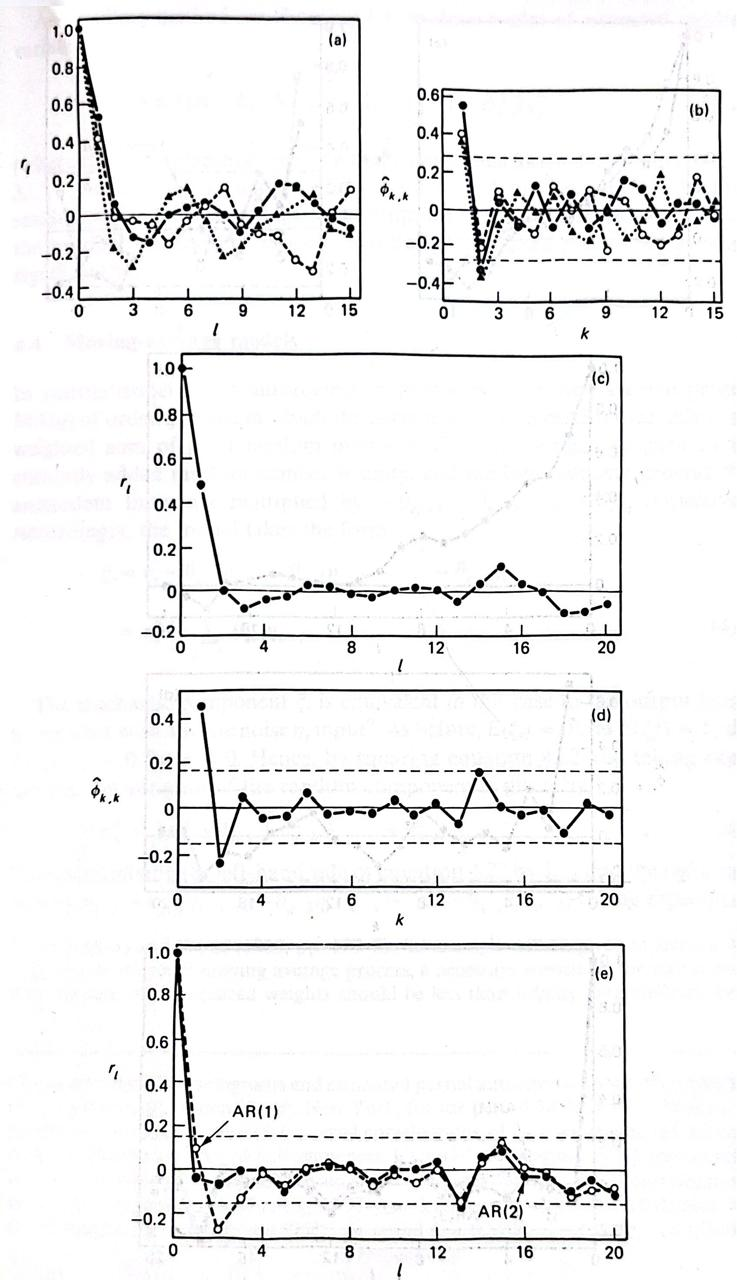
\includegraphics[width=1.1\linewidth]{fiKo43.jpeg}  % from Kotte (stochas)
    \end{center}
\end{minipage}
\end{frame}

%-------
% From Kotte (Stochastic WR tech)
\section{Moving average models}
\begin{frame}{Moving average models}
    In contrasting with \emph{autoregressive processes}, a \alert{moving-average process MA(q)} of order $q$ is one in which the current value of a random variable is the weighted sum of $q+1$ \emph{random numbers}. Here, the weight assigned to the currently added \emph{random number} is unity, and \emph{random numbers} generated at antecedent times are multiplied by $-\theta_{q,1}, -\theta_{q,2}, \cdots, -\theta_{q,q}$, respectively. Accordingly, the mode takes the form
    \begin{equation}
        \xi = \eta_t - \theta_{q,1} \eta_{t-1} - \theta_{q,2} \eta_{t-2}-\cdots- \theta_{q,q} \eta_{t-q} = \eta_t - \sum_{j=1}^q \theta_{q,j} \eta_{t-j}  
        \label{e422}
    \end{equation}
    The stochastic component $\xi_t$ is equivalent in this case to the output from \emph{linear filter} with a \emph{white noise } $\eta_t$ input. As before, $E[\xi_t] = 0$ and $E[\xi_t^2] =1$; also, $E[\eta_t \eta_{t-k}]=0$ for $k\neq 0$. Hence, by squaring the equation~\ref{e422} and taking expectations,the variance of the random component is given by
    \begin{equation}
        \sigma_{\eta}^2 = \frac{1}{1+\theta_{q,1}^2 + \theta_{q,2}^2 + \cdots + \theta_{q,q}^2}
        \label{e423}
    \end{equation}
    Then multiplying the left-hand side of equation~\ref{e422} by $\xi_{t-k}$ and the right-hand side by $\eta_{t-k} -\theta_{q,1}\eta_{t-1-k} - \theta_{q,2}\eta_{t-2-k} - \cdots -\theta_{q,q}\eta_{t-q-k}$, taking expectations and substituting for $\sigma_{\eta}^2$ from equation~\ref{e423}, we obtain
    \begin{equation}
        \rho_k = \frac{-\theta_{q,k} + \theta_{q,1}\theta_{q,k+1} + \theta_{q,2}\theta_{q,k+2}+ \cdots + \theta_{q, q-k}\theta_{q,q}}{1+\theta_{q,1}^2 + \theta_{q,2}^2 + \cdots + \theta_{q,q}^2 }, \quad \quad k =1,2,3,\cdots, q
        \label{e424}
        \end{equation}
        and $\rho_k = 0$, $k > q$, where $\rho_k$ is the lag-k \emph{autocorrelation coefficient}.
\end{frame}

\begin{frame}{Moving average models}
    For the \emph{first-order moving-average model MA(1)}, therefore
    \begin{equation}
        \rho_1 = \frac{-\theta_{1,1}}{1+\theta_{1,1}^2}
        \label{e425}
        \end{equation}
        Hence, $\theta_{1,1}$ can be estimated from the roots of the equation
    \begin{equation}
        \hat{\theta}_{1,1}^2 + \frac{\hat{\theta}_{1,1}}{r_1} + 1 = 0
        \label{e426}
        \end{equation}
        It is seen that one root is the reciprocal of the other and the root which satisfies the \emph{invertibility} constraint $|\hat{\theta}_{1,1}|>1$ is the initial estimate of the \emph{moving-average parameter}. However, such an estimate is found to be inefficient, this means that, for some other value of $\theta_{1,1}$, generated data could look more like the historical data. The suggested procedure is to estimate $\theta_{1,1}$ by minimizing the sum of squares of the residuals which is $\sum_{t=1}^N \tilde{\varepsilon}_t^2$, where $\tilde{\varepsilon}_1 = \tilde{\xi}_1$, $\tilde{\varepsilon}_2 = \tilde{\xi}_2 + \theta_{1,1}\tilde{\varepsilon}_1$, $\tilde{\varepsilon}_3 = \tilde{\xi}_3+ \theta_{1,1} \tilde{\varepsilon}_2$ and $\tilde{\xi}_t$, $t=1,2,3,\cdots, N$, is an observed sequence. The alternative ML procedure is much more difficult for estimation. 
\end{frame}

%-------
% From Kotte (Stochastic WR tech)
\section{Box-Jenkins models: formulation and identification}
\begin{frame}{Box-Jenkins models: formulation and identification}
    \begin{block}{Generalities}
    \end{block}
    The models described so far are special types of the so-called \alert{Box-Jenkins class of models}. Of these, the \alert{ARMA} model, which includes the \emph{autoregressive}, the \emph{moving-average} and the mixed types, is commonly applied to \emph{stationary} time series.

    A \emph{backshift} operator $B$ is used in defining the models, so that by using the previous notation $B\xi_t = \xi_{t-1}$, $B^2 \xi_t = \xi_{t-2}$ and in general $B^p \xi_t = \xi_{t-p}$. Likewise, $B^q \eta_t = \eta_{t-q}$. There is also a difference operator $\nabla$ such that $\nabla \xi_t = (1-B)\xi_t = \xi_t - \xi_{t-1}$, $\nabla^2 \xi_t = (1-B)^2 \xi_t = (\xi_t - \xi_{t-1})-(\xi_{t-1}-\xi_{t-2}) = \xi_t - 2 \xi_{t-1} + \xi_{t-2}$ and in general $\nabla^d \xi_t = (1-B)^d \xi_t$. This operator is useful in transforming a \emph{non-stationary} series  to one that is \emph{stationary}.  

    With this notation, \emph{AR(1)} and \emph{MA(1)} models are $(1-\phi_{1,1}B)\xi_t = \eta_t$ and $\xi_t = (1-\theta_{1,1}B)\eta_t$, respectively. Because these are equivalent to $\xi_t = (1-\phi_{1,1}B)^{-1} \eta_t = (1-\theta_{\infty,1} - \theta_{\infty,2} - \cdots)\eta_t$ and $(1-\theta_{1,1}B)^{-1} \xi_t = (1-\phi_{\infty,1} - \phi_{\infty,2} - \cdots)\xi_t = \eta_t$, respectively, it follows that $AR(1)\equiv MA(\infty)$ and $MA(1) \equiv AR(\infty)$. 

    The next important requirement is a methodology for identifying the type of model which adequately represents an observed sequence. This means that we should be able to make the best possible choice from the \emph{autoregressive}, \emph{moving-average} and \emph{mixed } models. 
    
\end{frame}

\begin{frame}{Box-Jenkins models: formulation and identification}
    \begin{block}{Autoregressive moving-average (ARMA(p,q)) model}
    \end{block}
     The mixed \alert{autoregressive moving-average (ARMA(p,q)) model} is specified by combining equations~\ref{e41} and ~\ref{e422}   
     \begin{equation}
            \xi_t = \phi_{p,1} \xi_{t-1} + \phi_{p,2} \xi_{t-2} + \cdots + \phi_{p,p} \xi_{t-p} + \eta_t - \theta_{q,1} \eta_{t-1} - \theta_{q,2} \eta_{t-2}-\cdots- \theta_{q,q} \eta_{t-q} 
            \label{e427}
        \end{equation}
        For instance the effect of \emph{linear aquifers} and \emph{independent rainfall} amounts justifies the approximate representation of \emph{river flow processes} through \emph{ARMA} models. They are also analogous to those \emph{conceptual models} in \emph{parametric hydrology} that are based on \emph{linear reservoirs}. The equation~\ref{e427} can be written as
        \begin{equation}
            \phi_p (B) \xi_t = \theta_q (B) \eta_t
            \label{e428}
        \end{equation}
        where 
        \begin{equation}
            \phi_p (B) = 1- \phi_{p,1} B - \phi_{p,2} B^2 - \cdots - \phi_{p,p} B^p
            \label{e429}
        \end{equation}
        and
        \begin{equation}
            \theta_q (B) = 1- \theta_{q,1} B - \theta_{q,2} B^2 - \cdots - \theta_{q,q} B^q
            \label{e430}
        \end{equation}
        Equations~\ref{e429} and ~\ref{e430} represent two polynomials of order $p$ and $q$ respectively. The prerequisites for \emph{stationarity} and \emph{invertibility}  respectively are that the roots of the equations $\phi_p (B) =0$ and $\theta_q (B) =0$ or that these roots, which are also termed the zeros of $B$, should lie \emph{outside} the \emph{unit circle} (these conditions are applicable to \emph{AR(p)} and \emph{MA(q)} processes respectively). Note that the estimation of the parameters of the \emph{ARMA(p,q)} mode is not a straightforward procedure. \alert{Parsimony} must be follow in order to get the minimum $p+q$ parameters. 
\end{frame}
 
\begin{frame}{Box-Jenkins models: formulation and identification}
    \begin{block}{Autoregressive moving-average (ARMA(1,1)) model}
    \end{block}
    In the class of \emph{mixed models}, the simplest is the \emph{ARMA(1,1)} model 
    \begin{equation}
        \xi_t  = \phi_{1,1}\xi_{t-1} + \eta_t - \theta_{1,1} \eta_{t-1}
        \label{e431}
    \end{equation}
    Let $E[\eta_t] = E[\xi_t] = 0$, $E[\xi_t^2] = 1$, $\rho_k = E[\xi_t \xi_{t-k}]$ and $E[\xi_t \eta_{t-1}] = \rho_{\xi, \eta} (-1)$. As noted before, $E[\eta_t \eta_{t-k}]=0$ for $k \neq 0$ and $E[\eta_t  \xi_{t-k}]=0$ for any integer $k>0$. Initially, if equation~\ref{e431} is multiplied by $\xi_t$ and expectations are taken, it follows that
    \begin{equation}
        \begin{aligned}
            1 &= \phi_{1,1}\rho_1 + E[\eta_t(\phi_{1,1} \xi_{t-1} + \eta_t - \theta_{1,1} \eta_{t-1})] - \theta_{1,1} \rho_{\xi, \eta} (-1) \\
              &= \phi_{1,1} \rho_1 + \sigma_{\eta}^2 - \theta_{1,1} \rho_{\xi, \eta} (-1)
        \end{aligned}
        \label{e432}
    \end{equation}
    Then, by multiplying equation~\ref{e431} by $\eta_{t-1}$ and $\xi_{t-1}$ in turn and taking expectations
    \begin{equation}
        \rho_{\xi, \eta} (-1) = (\phi_{1,1} - \theta_{1,1}) \sigma_{\eta}^2
        \label{e433}
    \end{equation}
    and
    \begin{equation}
        \rho_{1} = \phi_{1,1} - \theta_{1,1} \sigma_{\eta}^2
        \label{e434}
    \end{equation}
    Hence 
    \begin{equation}
        \sigma_{\eta}^2 =  \frac{1-\phi_{1,1}^2}{1+\theta_{1,1}^2 - 2\phi_{1,1} \theta_{1,1}}
        \label{e435}
    \end{equation}
    and
    \begin{equation}
        \rho_{1} = \frac{(1-\phi_{1,1}\theta_{1,1})(\phi_{1,1}- \theta_{1,1})}{1+\theta_{1,1}^2 - 2\phi_{1,1}\theta_{1,1}}
        \label{e436}
    \end{equation}

\end{frame}

\begin{frame}{Box-Jenkins models: formulation and identification}
    \begin{block}{Autoregressive moving-average (ARMA(1,1)) model}
    \end{block}
    Also, by multiplying equation~\ref{e431} by $\xi_{t-k}$, where $k\geq 2$, and by taking expectations
    \begin{equation}
        \rho_{k} = \phi_{1,1} \rho_{k-1}
        \label{e437}
    \end{equation}
    An initial estimate $\hat{\phi}_{1,1}$ of $\phi_{1,1}$ is obtained from $r_2 / r_1$ (where $r_1$ and $r_2$ are the lag-one and lag-two serial correlation coefficients) by using equation~\ref{e437}. The substitution of $\hat{\phi}_{1,1}$ and $r_1$ in equation~\ref{e436} gives an initial estimate $\hat{\theta}_{1,1}$ of $\theta_{1,1}$. Then, given the \emph{stationarity} and \emph{invertibility} constraints $-1<\phi_{1,1}, \theta_{1,1}<1$ a \emph{grid search} is made, and the two parameters are estimated by minimising the sum of squares of residuals which is $\sum_{t=1}^N \tilde{\varepsilon}_t^2$, where $\tilde{\varepsilon}_1=\tilde{\xi}_1$, $\tilde{\varepsilon}_2=\tilde{\xi}_2 - \phi_{1,1}\tilde{\xi}_1 + \theta_{1,1} \tilde{\varepsilon}_1$, $\tilde{\varepsilon}_3=\tilde{\xi}_3 - \phi_{1,1}\tilde{\xi}_2 + \theta_{1,1} \tilde{\varepsilon}_2$, $\cdots$, and $\tilde{\xi}_t$, $t=1, 2, 3, \cdots, N$ is an observed sequence.

\end{frame}

\begin{frame}{Box-Jenkins models: formulation and identification}
    \begin{block}{Autoregressive integrated moving-average (ARIMA(p,d,q)) model}
    \end{block}
    The \alert{ARIMA} model is a generalized version of the \emph{ARMA} model which can account for non-stationarity behaviour by means of a dth-order difference operator $\nabla^d$. By using the notation explained above it can be represented by
    \begin{equation}
        \phi_p (B) \nabla^d \xi_t = \theta_q (B) \eta_t
        \label{e439}
    \end{equation}
    By changing the variable $\xi_t$, this can be transformed to an \emph{ARMA(p,q)} type. For example, if $\psi_t = \nabla^d \xi_t$,
    \begin{equation}
        \phi_p (B) \psi_t= \theta_q (B) \eta_t
        \label{e440}
    \end{equation}
    This means that, if $\phi(B)$ and $\theta(B)$ are defined by equations~\ref{e429} and ~\ref{e430}, respectively, the series $\psi_t$ is generated by an \emph{ARMA(p,q)} process; correspondingly, $\xi_t$ is of the \emph{ARIMA(p,d,q)} type. In practice, a \emph{minimum value} of $d$ is found so that the process given by equation~\ref{e440} satisfies the necessary constraints. As Box and Jenkins postulate, the parameters $p$, $d$ and $q$ need not be greater that 2 for practical purposes. 
    
    Consider the case when $\xi_t$ is generated by an \emph{ARIMA(1,1,1)} process. Initially, the non-stationary series $\xi_t$ is transformed into a stationary series $\psi_t$ by differencing as $\psi_t = \xi_t - \xi_{t-1}$. Then the parameters of \emph{ARMA(1,1)} model are estimated. An \emph{ARIMA(2,2,2)} process can be similarly investigated by replacing $\psi_t = \xi_t -2\xi_{t-1} + \xi_{t-2}$ in equation~\ref{e440}. 
\end{frame}

\begin{frame}{Box-Jenkins models: formulation and identification}
    \vspace{-5pt}
    \begin{block}{Model identification and estimation}
    \end{block}
\begin{minipage}[]{0.59\textwidth}
        \begin{itemize}
            \item An iterative procedure for fitting \emph{Box-Jenkins} model is given in the figure. This procedure is performed recursively, where the essential steps are \emph{identification}, \emph{estimation} and \emph{verification} of the model \emph{type}, \emph{order} and \emph{parameters}. 
            \item The \emph{serial correlogram} ($\rho_i$) is the initial requirement. Also, the estimation of the \emph{partial autocorrelation} ($\phi_{i,i}$) is equally important. 
            \item  Note that complications arise from unremoved non-stationary effects. This can be identified in the \emph{serial correlogram} and in the \emph{partial autocorrelation}.
            \item The behaviour of \emph{acf} and \emph{pcf} functions are different. For instance, in the \emph{AR(1)} model, the \emph{acf} decrease exponentially, whereas the \emph{pcf} are theoretically zero exept for $\phi_{1,1} \neq 0$. The situation is the opposite for a \emph{MA(1)} model. 
            \item In an \emph{ARMA(1,1)} process, both functions decay exponentially after $k=1$. For identifying these and other types, see following table. 
        \end{itemize}
\end{minipage}
\hfill
\begin{minipage}[]{0.40\textwidth}
    \begin{center}
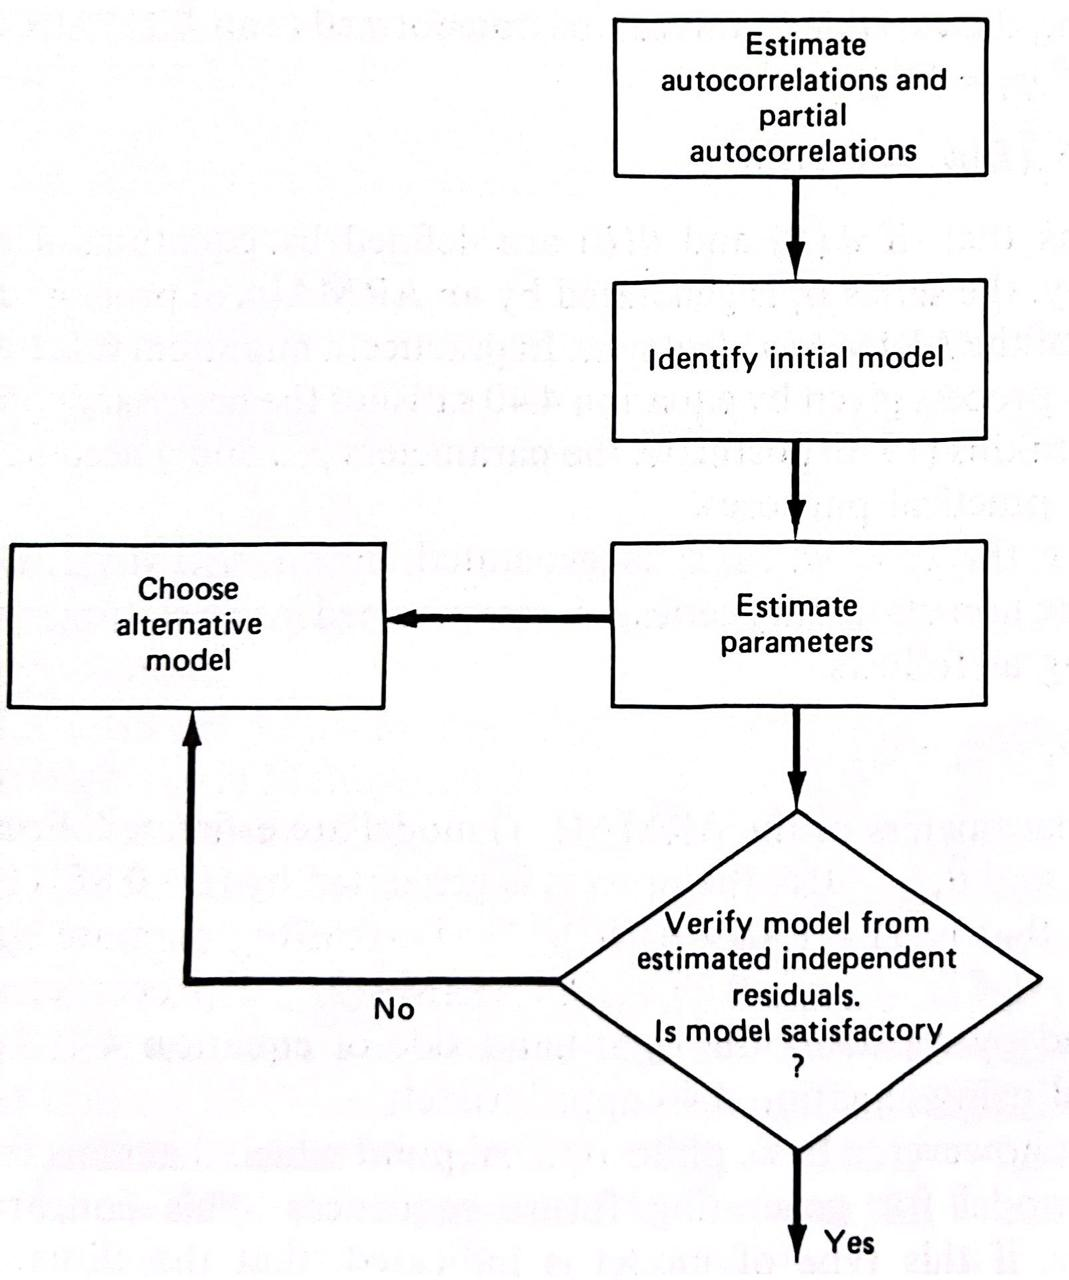
\includegraphics[width=1.1\linewidth]{fiKo46.jpeg}  % from Kotte (stochas)
    \end{center}
\end{minipage}
\end{frame}

 \begin{frame}{Box-Jenkins models: formulation and identification}
    \begin{block}{Model identification and estimation}
    \end{block}
    \begin{center}
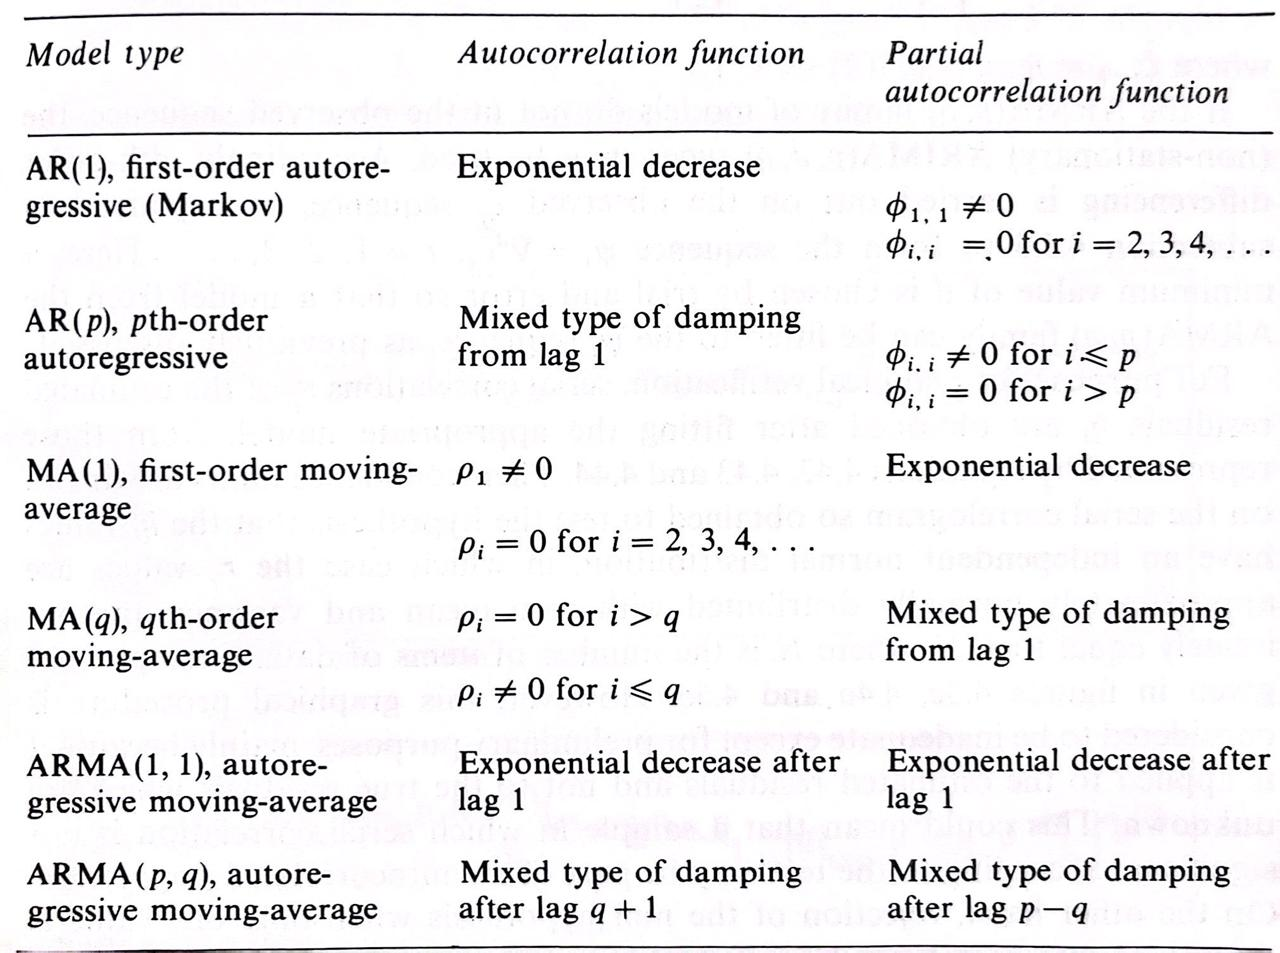
\includegraphics[width=1\linewidth]{taKo41.jpeg}  % from Kotte (stochas)
    \end{center}
\end{frame}
 

 \begin{frame}{Box-Jenkins models: formulation and identification}
    \begin{block}{Model identification and estimation}
    \end{block}
    \begin{enumerate}
        \item The shapes of the sample \emph{acf} and \emph{pcf} functions are examined for practical identification purposes. 
        \item If  the indications are that the process is an \emph{autoregressive} type, a \emph{significance test} is made to determine its order. This is based on the assumption that the estimated \emph{pcf} function $\hat{\phi}_{i,i}$, $i>p$, of an \emph{AR(p)} process are normally distributed with zero mean and variance  $1/N$, where $N$ is the number of observations. Similarly, for an \emph{MA(q)} process, the \emph{serial correlation} $r_l$, $l>q$, are taken to be \emph{normally distributed}  with zero mean and variance 
            \begin{equation}
                Var(r_l) \approx \frac{\left( 1+2\sum_{k=1}^q r_k^2 \right)}{N} \quad \quad l > q
            \end{equation}
        \item Estimate the parameters of the model according to the procedure explained before. 
        \item After \emph{identification} and \emph{estimation}, \emph{diagnostic checking} or \emph{verification} is made by testing the residuals thus obtained for independence. For general \emph{ARMA(p,q)} model described as
            \[
                \phi (B) \xi_t = \theta (B) \eta_t
            \]
            the estimated residuals are, therefore $\hat{\eta}_t = \hat{\theta}^{-1} (B) \hat{\phi} (B) \hat{\xi}_t$, where $\hat{\theta}$ and $\hat{\phi}$ are polynomials (in $B$) in which the coefficients are estimated parameters, and $\hat{\xi}_t$, $t=1,2,3,\cdots,N$, is an observed sequence. 
   \end{enumerate}
\end{frame}

 \begin{frame}{Box-Jenkins models: formulation and identification}
    \begin{block}{Model identification and estimation}
    \end{block}
    \begin{enumerate}
        \item To clarify this, consider a \emph{pth-order autoregressive model} $\phi(B) \xi_t = \eta_t$ given explicitly by equation~\ref{e41}. In this case, the \emph{residuals} are estimated as follow
            \begin{equation}
                \tilde{\eta}_t = \tilde{\xi}_t - \sum_{k=1}^p \hat{\phi}_{p,k} \tilde{\xi}_{t-k}
                \label{e442}
            \end{equation}
  
            where $\tilde{\xi}_{t-k} = 0$, if $t-k <1$. Like wise for the \emph{moving-average model} given by equation~\ref{e422}, estimated \emph{residuals} are found from 
            \begin{equation}
                \tilde{\eta}_t = \tilde{\xi}_t + \sum_{k=1}^q \hat{\theta}_{q,k} \tilde{\eta}_{t-k}
                \label{e443}
            \end{equation}
            where $\tilde{\eta}_{t-k} = 0$, if $t-k < 1$. Similarly, the estimated \emph{residuals} obtained by applying the \emph{ARMA(p,q)} model are given by
\begin{equation}
                \tilde{\eta}_t = \tilde{\xi}_t - \sum_{k=1}^p \hat{\phi}_{p,k} \tilde{\xi}_{t-k} + \sum_{k=1}^q \hat{\theta}_{q,k} \tilde{\eta}_{t-k}
                \label{e444}
            \end{equation}
            where $\tilde{\xi}_{t-k} =\tilde{\eta}_{t-k} = 0$, if $t-k < 1$.
    \end{enumerate}
\end{frame}

 \begin{frame}{Box-Jenkins models: formulation and identification}
    \begin{block}{Model identification and estimation}
    \end{block}
    \begin{itemize} 
        \item If the \emph{ARMA(p,q)} family of models do not fit the observed sequence, the (non-stationary) \emph{ARIMA(p,d,q)} types may be tried. Accordingly, dth-order differencing is carried out on the observed $\tilde{\xi}_t$ sequence, as explained in before to form the sequence $\tilde{\psi}_t = \nabla^d \xi_t$, $t=1,2,3, \cdots$. Here, a minimum value of $d$ is chosen by trial and error so that a model from the \emph{ARMA(p,q)} family can be fitted to the $\tilde{\psi}_t$ sequence, as previously discussed. 
        \item For the purpose of graphical verification, \emph{serial correlations} $r_l$ of the estimated residuals $\tilde{\eta}_t$ are obtained after fitting the appropriate model from those represented by equations~\ref{e442}, ~\ref{e443} and ~\ref{e444}. The \emph{confidence limits} are drawn on the \emph{serial correlogram} so obtained to test the hypothesis that the $\tilde{\eta}_t$ values have an independent \emph{normal distribution}, in which case the $r_l$ values are approximately \emph{normally distributed} with zero mean and variance approximately equal to $1/N$, where $N$ is the number of data.  
    \end{itemize} 
\end{frame}
 
\end{document}
